\documentclass[fleqn,10pt]{wlscirep}
\usepackage[utf8]{inputenc}
\usepackage[T1]{fontenc}
\usepackage[section]{placeins}
\usepackage{amsmath}
\usepackage{lineno}
\usepackage{float}
\usepackage{booktabs}
\usepackage{longtable}
\usepackage{array}
\usepackage{multirow}
\usepackage{wrapfig}
\usepackage{colortbl}
\usepackage{pdflscape}
\usepackage{tabu}
\usepackage{threeparttable}
\usepackage{threeparttablex}
\usepackage[normalem]{ulem}
\usepackage{makecell}
\usepackage{xcolor}
\linenumbers

\providecommand{\tightlist}{%
  \setlength{\itemsep}{0pt}\setlength{\parskip}{0pt}}

\usepackage{color}
\usepackage{fancyvrb}
\newcommand{\VerbBar}{|}
\newcommand{\VERB}{\Verb[commandchars=\\\{\}]}
\DefineVerbatimEnvironment{Highlighting}{Verbatim}{commandchars=\\\{\}}
% Add ',fontsize=\small' for more characters per line
\usepackage{framed}
\definecolor{shadecolor}{RGB}{248,248,248}
\newenvironment{Shaded}{\begin{snugshade}}{\end{snugshade}}
\newcommand{\AlertTok}[1]{\textcolor[rgb]{0.94,0.16,0.16}{#1}}
\newcommand{\AnnotationTok}[1]{\textcolor[rgb]{0.56,0.35,0.01}{\textbf{\textit{#1}}}}
\newcommand{\AttributeTok}[1]{\textcolor[rgb]{0.77,0.63,0.00}{#1}}
\newcommand{\BaseNTok}[1]{\textcolor[rgb]{0.00,0.00,0.81}{#1}}
\newcommand{\BuiltInTok}[1]{#1}
\newcommand{\CharTok}[1]{\textcolor[rgb]{0.31,0.60,0.02}{#1}}
\newcommand{\CommentTok}[1]{\textcolor[rgb]{0.56,0.35,0.01}{\textit{#1}}}
\newcommand{\CommentVarTok}[1]{\textcolor[rgb]{0.56,0.35,0.01}{\textbf{\textit{#1}}}}
\newcommand{\ConstantTok}[1]{\textcolor[rgb]{0.00,0.00,0.00}{#1}}
\newcommand{\ControlFlowTok}[1]{\textcolor[rgb]{0.13,0.29,0.53}{\textbf{#1}}}
\newcommand{\DataTypeTok}[1]{\textcolor[rgb]{0.13,0.29,0.53}{#1}}
\newcommand{\DecValTok}[1]{\textcolor[rgb]{0.00,0.00,0.81}{#1}}
\newcommand{\DocumentationTok}[1]{\textcolor[rgb]{0.56,0.35,0.01}{\textbf{\textit{#1}}}}
\newcommand{\ErrorTok}[1]{\textcolor[rgb]{0.64,0.00,0.00}{\textbf{#1}}}
\newcommand{\ExtensionTok}[1]{#1}
\newcommand{\FloatTok}[1]{\textcolor[rgb]{0.00,0.00,0.81}{#1}}
\newcommand{\FunctionTok}[1]{\textcolor[rgb]{0.00,0.00,0.00}{#1}}
\newcommand{\ImportTok}[1]{#1}
\newcommand{\InformationTok}[1]{\textcolor[rgb]{0.56,0.35,0.01}{\textbf{\textit{#1}}}}
\newcommand{\KeywordTok}[1]{\textcolor[rgb]{0.13,0.29,0.53}{\textbf{#1}}}
\newcommand{\NormalTok}[1]{#1}
\newcommand{\OperatorTok}[1]{\textcolor[rgb]{0.81,0.36,0.00}{\textbf{#1}}}
\newcommand{\OtherTok}[1]{\textcolor[rgb]{0.56,0.35,0.01}{#1}}
\newcommand{\PreprocessorTok}[1]{\textcolor[rgb]{0.56,0.35,0.01}{\textit{#1}}}
\newcommand{\RegionMarkerTok}[1]{#1}
\newcommand{\SpecialCharTok}[1]{\textcolor[rgb]{0.00,0.00,0.00}{#1}}
\newcommand{\SpecialStringTok}[1]{\textcolor[rgb]{0.31,0.60,0.02}{#1}}
\newcommand{\StringTok}[1]{\textcolor[rgb]{0.31,0.60,0.02}{#1}}
\newcommand{\VariableTok}[1]{\textcolor[rgb]{0.00,0.00,0.00}{#1}}
\newcommand{\VerbatimStringTok}[1]{\textcolor[rgb]{0.31,0.60,0.02}{#1}}
\newcommand{\WarningTok}[1]{\textcolor[rgb]{0.56,0.35,0.01}{\textbf{\textit{#1}}}}

\newlength{\cslhangindent}
\setlength{\cslhangindent}{1.5em}
\newenvironment{CSLReferences}%
{\setlength{\parindent}{0pt}%
\everypar{\setlength{\hangindent}{\cslhangindent}}\ignorespaces}%
{\par}

\title{Multiorder Hydrologic Position in Europe as a Set of Metrics in Support of Machine Learning Based Groundwater Mapping at Regional and National Scales}

\author[*, 1]{Maximilian Nölscher}
\author[2]{Michael Mutz}
\author[1]{Stefan Broda}
\affil[1]{Federal Institute for Geosciences and Natural Resources (BGR), Sub-Department: Basic information Groundwater and Soil (B2.2), Berlin, 13593, Germany}
\affil[2]{independent researcher}
\affil[*]{corresponding author: Maximilian Nölscher (max-n@posteo.de)}


\begin{abstract}
This dataset (EU-MOHP v013.1.0) provides information on the multiorder hydrologic position of a geographic point within its respective river network and catchment as gridded maps. More precisely, it comprises the three measures ``lateral position'' as a relative measure of the position between the stream and the catchment boundary/ watershed, ``divide stream distance'' as an absolute distance measure that serves as a proxy for the position within the catchment and ``stream distance'' as an absolute measure of the distance to the nearest stream. These three measures were calculated for several hydrologic orders to reflect different spatial scales. Its spatial extent covers major parts of physiographical Europe or the European Economic Area (EEA39). Although there might be many potential use cases, this dataset serves predominantly as valuable static geophysical or environmental predictor variable among other input data for mapping or regionalization tasks in the context of hydrogeology and hydrology using machine learning.
\end{abstract}
\begin{document}

\flushbottom
\maketitle
%  Click the title above to edit the author information and abstract

\thispagestyle{empty}

\hypertarget{background-summary}{%
\section{Background \& Summary}\label{background-summary}}

In recent years, data science tools such as machine learning are increasingly applied to and specifically developed for hydro(geo)logical challenges and research questions \cite{zounemat-kermani_neurocomputing_2020}. In the field of hydrogeology, machine learning has been used successfully for groundwater level prediction and a variety of mapping tasks \cite{desimone_machine-learning_2020, knoll_large_2019, knoll_nation-wide_2020, mueller_surrogate_2019, stackelberg_machine_2021, wang_comparison_2016, wunsch_forecasting_2018, wunsch_groundwater_2020}. Since machine learning models -- except for hybrid- or physically-based models -- are purely based on data with no built-in knowledge of physical processes, it is important to provide as many features (synonyms: predictor variables, explanatory variables) as possible that have an impact on the target variable to potentially enable the machine learning algorithm to approximate the underlying process. For surface and near-surface processes, this criterion can be more or less fulfilled by the availability of remote sensing data, whereas for modelling subsurface processes such as in hydrogeology, this poses a serious challenge.

The key motivation for this dataset is to provide a set of features that introduce hydrological context to machine learning models regarding the horizontal position of a point within its catchment. Therefore, it serves as a proxy for multiple geophysical characteristics of a hydrologic system. It complements commonly available datasets and tackles the above mentioned challenge.
This dataset is strongly inspired by Belitz et al.~(2019) and adapts their ideas and methods to the ``EU-Hydro - River Network Database'' but --- in contrast --- using purely free open source software and a strong focus on reproducibility \cite{belitz_multiorder_2019}. Belitz et al.~(2019) provide a comprehensive explanation of the motivation as well as a detailed discussion for further reading \cite{belitz_multiorder_2019}.

In their study, Belitz et al.~(2019) also provide the results from case studies to prove that the multiorder hydrologic position is a valuable feature when mapping diverse geophysical targets using machine learning \cite{belitz_multiorder_2019}. Its benefit to the performance of machine learning models has also been acknowledged by several other studies \cite{degnan_relation_2020, knierim_using_2020, stackelberg_machine_2021}.

Being a static geophysical catchment attribute, the EU-MOHP dataset can be used as features in any machine learning task in the domain of hydrology and hydrogeology. Because of the calculation based on the different stream orders, this dataset can be applied at multiple spatial scales and depths -- from local via regional to continental scales. Examples of use cases might be the mapping of hydrogeochemical parameters or hydraulic variables like depth to groundwater, the prediction of groundwater levels or catchment classification tasks using unsupervised machine learning methods.

The EU-MOHP v013.1.0 dataset comprises the 3 measures

\begin{itemize}
\tightlist
\item
  lateral position (LP)
\item
  divide stream distance (DSD) and
\item
  stream distance (SD)
\end{itemize}

for each of the 6 stream orders which leads to \(n_{measures}\cdot n_{streamorders} = 18\) different metrics to be used as features. Spatially, the dataset covers major parts of physiographical Europe and all of the 39 countries in the European Economic Area (EEA39). More precisely, it covers the 2 largest coherent land masses of the EEA39 (Fig. \ref{fig:studyareafigure}).

Conceptually, the three measures LP, DSD and SD of EU-MOHP are based on the idea that the location in hydrologic systems matters. A location can be e.g.~close to the confluence of two large rivers or in another extreme close the catchment boundary of headwater streams. The location or hydrologic position refers to the position of a point between a stream and its divide/catchment boundary. Thiessen divides were used as catchment boundaries instead of divides that are generated from digital elevation models. One major advantage is that Thiessen divides can be calculated purely based on the river network itself while avoiding issues such as closed lows in the resulting metrics \cite{belitz_multiorder_2019}. A Thiessen divide is the outline of a Thiessen catchment which is the area that contains all points to which a stream is closer than any other stream \cite{johnston_evaluation_2009}. In other words, a Thiessen divide contains all points with equal distance to the two nearest streams.

The overall concept also includes the spatial scale that the role of different hydrologic processes can depend upon. This issue is addressed by calculating the EU-MOHP measures for different hydrologic orders which are derived from the stream orders of the river network. For a specific hydrologic order \(i\), only streams with a stream order \(>= i\) were used (e.g.~for stream order 2, all streams with stream order 2, 3, 4 and greater, compare Fig. \ref{fig:schematicmohp}A and B). Here, the stream orders are defined according to \cite{strahler_quantitative_1957} where all streams without tributaries are assigned to the first stream order (headwater streams). The stream order downstream of a confluence increases by 1 if the upstream stream orders are equal. If the stream orders are not equal, it inherits the greater stream order. Therefore, each hydrologic order reflects a different scale.

Based on the river network and the Thiessen divides, the EU-MOHP measures (LP, DSD, SD) can be calculated as follows:

\begin{equation}
\text{LP}_i = \frac{\text{DS}_i}{\text{DS}_i + \text{DD}_i} \label{eq:eqlp}
\end{equation}

\begin{equation}
\text{DSD}_i = \text{DS}_i + \text{DD}_i \label{eq:eqdsd}
\end{equation}

\begin{equation}
\text{SD}_i = \text{DS}_i \label{eq:eqsd}
\end{equation}

\noindent
where \(i\) is the hydrologic order, \(DS\) is the horizontal distance to the nearest stream (Fig. \ref{fig:schematicmohp}) and \(DD\) is the horizontal distance to the nearest divide without crossing a stream (Fig. \ref{fig:schematicmohp}). This condition arises from the fact that water flows towards the topographically lowest points namely the streams.

Examples of the generated EU-MOHP v013.1.0 maps are shown in Fig. \ref{fig:datasetmapoverviewplot} for the two hydrologic orders 3 and 4.

\hypertarget{methods}{%
\section*{Methods}\label{methods}}
\addcontentsline{toc}{section}{Methods}

Most processing and calculation steps were done in the R programming language (Fig. \ref{fig:workflowfigure}C) \cite{r_core_team_r_2020}. Due to the memory size of this dataset as well as for the sake of computational speed, a PostgreSQL database with PostGIS extension was used for some processing steps of vector data and a GRASS GIS database was used for all final raster based calculations of the MOHP metrics (Fig. \ref{fig:workflowfigure}D and E). For reproducibility and programming reasons, all processing steps including the databases were tracked and executed through a data processing pipeline using the targets package in R (Fig. \ref{fig:workflowfigure}) \cite{landau_targets_2021}. More details can be found in the following sections or in the code itself (see \protect\hyperlink{code-availability}{Code availability}). This processing or targets pipeline can be seen as programming script that tracks each step and skips processing steps that are still up-to-date when re-running the script.

To better refer to the code during the description of the methods, each processing step provides the name of its related target in the targets pipeline and the file containing this target. Targets titled as \texttt{helper\ target} in the code are not described here because they are not relevant to the description of the methods and exist only for technical reasons. Column names appear in different notations, but are always clearly assignable. E.g. the column notation \texttt{OBJECT\_ID} is used in the underlying river network dataset. This notation was changed to \texttt{object\_id} in the code for consistency and error reduction reasons. Other notations are used for a better readability.

\hypertarget{directory-and-file-structure}{%
\subsection*{Directory and file structure}\label{directory-and-file-structure}}
\addcontentsline{toc}{subsection}{Directory and file structure}

The directory and file structure of the project folder containing all code and files to generate this dataset is summarized in Fig. \ref{fig:projectdirtree} as tree. Files and directories that are not relevant for describing the methods are not shown here. The file \texttt{config.yml} (line !!1) contains definitions of variables that are meant to be changed by a user before running the script. The most relevant variable is \texttt{cellsize} which sets the raster cell width of the resulting EU-MOHP gridded maps. Another important variable is \texttt{area} to switch between a test study area and the complete study area for all EEA39. The test study area reduces the calculation time for pipeline testing purposes. The folder \texttt{grassdata} (line !!2) contains the GRASS GIS databases. The file \texttt{macro\_mohp\_feature.Rproj} (line !!3) is the R project file. \texttt{output\_data} (line !!5) contains sub-directories where the final EU-MOHP gridded maps are written to. \texttt{R} (line 9) contains R scripts where custom functions and constants are defined. \texttt{renv} (line !!19) and the file \texttt{renv.lock} (line !!25) are related to the R package \texttt{renv} for improved reproducibility by managing R package dependencies. The R script \texttt{run\_pipeline.R} contains code to execute the targets pipeline that does all the data processing and calculations. \texttt{targets} (line !!27) contains the definition of all targets or processing steps of the pipeline. For overview reasons, it is split thematically across multiple files. \texttt{\_targets} (line !!35) is used by the targets package internally. The file \texttt{\_targets.R} (line !!39) sets up the processing pipeline and loads all dependencies.

The resulting EU-MOHP metrics (Fig. \ref{fig:workflowfigure}G) were written to the sub-directories ``divide\_stream\_distance,'' ``lateral\_position,'' ``stream\_distance'' of \texttt{output\_data} as gridded maps in the GeoTiff (.tif) file format. The data descriptor was written to \texttt{output\_data} in the LaTeX (.tex) and PDF (.pdf) file format.

\hypertarget{underlying-dataset}{%
\subsection*{Underlying dataset}\label{underlying-dataset}}
\addcontentsline{toc}{subsection}{Underlying dataset}

The generation of this dataset is based on two basic data products which are the \href{https://land.copernicus.eu/imagery-in-situ/eu-hydro/eu-hydro-river-network-database?tab=download}{``EU-Hydro -- River Network Database'' version v013} and \href{https://land.copernicus.eu/imagery-in-situ/eu-hydro/eu-hydro-coastline?tab=download}{``EU-Hydro -- Coastline'' version v013} with the advantage that the dependencies are low from a data point of view \cite{noauthor_eu-hydro_2021, noauthor_eu-hydro_2021-1}. Therefore, it is possible to transfer the methodology to other regions with only little effort. The Tab. \ref{tab:inputdata} provides an overview of the input data layers building the basis for generating or reproducing this dataset.

The ``EU-Hydro -- River Network Database'' as well as the ``EU-Hydro -- Coastline'' were manually downloaded from the Copernicus - Land Monitoring Service website (Fig. \ref{fig:workflowfigure}A) in GeoPackage (.gpkg) and in Shapefile (.shp) file format, respectively (Fig. \ref{fig:workflowfigure}B) \cite{noauthor_eu-hydro_2021, noauthor_eu-hydro_2021}. The river network data is split into 2 .gpkg files for each of 35 the major river basins. All unzipped files together have a size of approximately 14GB. The single .shp file containing the coastline has a size of 288MB.

\hypertarget{data-import}{%
\subsection*{Data import}\label{data-import}}
\addcontentsline{toc}{subsection}{Data import}

The river network comprises the layers `Canals\_l,' `Ditches\_l,' `River\_Net\_l' in the ``euhydro\_\textless name of the river basin\textgreater\_v013'' named .gpkg file of all river basins of the river network data. They are imported with the target ``river\_networks'' in ``import\_targets.R'' (Fig. \ref{fig:projectdirtree}, line !!29). The layer ``Canals\_l'' contains canals, which are defined as ``an artificial waterway with no flow, or a controlled flow, usable or built for navigation'' \cite{gallaun_eu-hydro_2019}. The layer ``Ditches\_l'' contains ditches, which are defined as ``an artificial waterway with no flow, or a controlled flow, usually unlined, used for draining or irrigating land'' \cite{gallaun_eu-hydro_2019}. The layer ``Rivers\_l'' contains rivers, which are defined as ``a naturally flowing watercourse'' \cite{gallaun_eu-hydro_2019}.

The surface water bodies are derived from the layer `InlandWater.' This layer is imported by the target ``inland\_waters'' in ``import\_targets.R'' and contains inland water defined as ``a large body of water entirely surrounded by land.'' \cite{gallaun_eu-hydro_2019}. In this step, all geometries with an area smaller than \(4 \cdot Cellsize = 3600m^2\), where \(Cellsize\) is the area of raster cells, are removed. The polygon geometries of wider river parts were not included in the surface water bodies.

The river basins are based on the layer ``\textless name of river basin\textgreater\_eudem2\_basins\_h1'' in the ``drainage\_network\_\textless name of the river basin\textgreater\_public\_beta\_v009'' named .gpkg file. This layer is imported with the target ``river\_basins'' in ``studyarea\_targets.R'' (Fig. \ref{fig:projectdirtree}, line !!32) and contains polygon geometries of all sub-basins of a basin. The spatial coverage of the river basins is the basis for the study area. The study area itself delineates the area for which the EU-MOHP metrics will be calculated.

The fourth required data layer is the coastline. It is imported with the target ``coastline\_grouped'' in ``studyarea\_targets.R'' (Fig. \ref{fig:projectdirtree}, line !!32).

In this study, we used the coordinate reference system (CRS) ETRS89-extended / LAEA Europe with the EPSG code 3035. Therefore, all data was reprojected to this CRS after importing if necessary.

\hypertarget{preprocessing}{%
\subsection{Preprocessing}\label{preprocessing}}

\hypertarget{river-basins-study-area}{%
\subsubsection*{River Basins/ Study Area}\label{river-basins-study-area}}
\addcontentsline{toc}{subsubsection}{River Basins/ Study Area}

Firstly, the preprocessing steps related to the river basins are described because they aim at the determination of a study area, which is required for subsequent processing steps. This study area also serves as a basis for which the EU-MOHP measures are calculated. The following steps refer to targets that can be found in the file ``studyarea\_targets.R'' (Fig. \ref{fig:projectdirtree}, line !!32). After the previously mentioned import, the sub-basins were unioned basin-wise (target: river\_basins\_unioned). Then, all polygons belonging to European oversea territories such as the French islands in the Caribbean were removed (target: river\_basins\_subset). The resulting polygon geometries were unioned in the PostgreSQl database (target: river\_basins\_subset\_union\_in\_db). The PostgreSQl database has reduced the run-time of the union drastically compared to R. The polygon geometries have a large amount of nodes due to the high details in the digitized coastline which causes long run-times in R. Subsequently, out of these polygons of contiguous land masses the 10 area-wise largest polygons were chosen as study area (target: river\_basins\_region\_name). Lastly, names were assigned to each of the polygons (target: selected\_studyarea).

\hypertarget{river-network}{%
\subsubsection*{River Network}\label{river-network}}
\addcontentsline{toc}{subsubsection}{River Network}

After the data import, the next step is the filtering of linestring geometries from the river network based on attribute columns \texttt{DFDD} and \texttt{HYP} (target: river\_networks\_non\_dry\_selected\_streamtypes in ``preprocessing\_targets.R'' file; Fig. \ref{fig:projectdirtree}, line 30). \texttt{DFDD} classifies the geometries into BH140 (river), BH020 (canal) and BH030 (ditch). Canals and ditches were removed from the river network by only keeping the geometries with the value ``BH140'' for several reasons. Many of the canal and ditch geometries have missing stream order values, which is required for the following processing steps. Another reason is the assumption that canals might be hydraulically disconnected to the natural hydrologic system through walls with low permeability. Lastly, the overall importance of canals and ditches is low when comparing the number of geometries to rivers as shown in Fig. \ref{fig:dfddstatsbarplot}. !!The section \protect\hyperlink{technical-validation}{Technical Validation} provides a discussion on this issue. \texttt{HYP} classifies the geometries into the following degrees of hydrologic persistence: 1 (Perennial), 2 (Intermittent), 3 (Ephemeral) and 4 (Dry). Geometries with the value 4 (Dry) were removed. Then, missing and invalid stream order values are imputed the with the value 1 to include them in the first hydrologic order (target: river\_networks\_imputed\_streamorder\_canals\_as\_1). The river network geometries were clipped to the study area by only keeping geometries that intersect with the study area (target: db\_river\_networks\_strahler\_studyarea).

The next processing step implements a method to obtain linestring geometries that represent the mainstems of the rivers and its tributaries (target: rivernetworks\_merged\_per\_streamorder). This is achieved by merging the geometries by a column containing an unique id for each mainstem. The mainstem is defined here as the longest path from the head water to the most distant river mouth (see geometries with the same \texttt{Levelpath\ ID} in Fig. \ref{fig:mainstemscheme}B). As the underlying river network data has no column providing this information, it is necessary to first generate this id column by which we will conduct the merging of the lines (!!\cite{belitz_multiorder_2019} used the already existing column \texttt{LevelPathI} from their underlying river network dataset). For doing so, it is now required to first derive a river network for each hydrologic order separately. This is achieved by keeping only geometries with a stream order equal or greater than the specific hydrologic order as described in \protect\hyperlink{background-summary}{Background \& Summary}. The river networks of each individual hydrologic order was then sorted by column \texttt{LONGPATH} in descending order.

\footnotesize

\begin{Shaded}
\begin{Highlighting}[]
\NormalTok{river\_network\_path }\OtherTok{\textless{}{-}} 
\NormalTok{  river\_network }\SpecialCharTok{\%\textgreater{}\%} 
  \FunctionTok{as\_tibble}\NormalTok{() }\SpecialCharTok{\%\textgreater{}\%} 
  \FunctionTok{arrange}\NormalTok{(}\SpecialCharTok{{-}}\NormalTok{longpath) }\SpecialCharTok{\%\textgreater{}\%} 
  \FunctionTok{select}\NormalTok{(object\_id, nextdownid)}
\end{Highlighting}
\end{Shaded}

\normalsize

\texttt{LONGPATH} indicates the length of the path from the start node of a geometry to the end node of the most downstream geometry of the river network. Starting with the topmost geometry, all downstream geometries that constitute the longest path to the river mouth are identified by making use of the columns \texttt{OBJECT\_ID} and \texttt{NEXTDOWNID} and the R package \texttt{igraph}. This is the start of a loop over the sorted geometries. The column \texttt{OBJECT\_ID} provides an unique ID for every linestring geometry and \texttt{NEXTDOWNID} indicates the \texttt{OBJECT\_ID} of the next downstream geometry. Based on this information the function \texttt{subcomponent} of the \texttt{igraph} package identifies the \texttt{OBJECT\_ID}s of all geometries that belong the the longest path. These identified geometries were then removed from the river network for the next iteration of the loop. The subsequent iteration identifies all geometries downstream of the current topmost geometry of the remaining river network. This is repeated until the river network has no geometries left.

\footnotesize

\begin{Shaded}
\begin{Highlighting}[]
\NormalTok{longestpaths\_list }\OtherTok{\textless{}{-}} \FunctionTok{list}\NormalTok{()}
\NormalTok{i }\OtherTok{\textless{}{-}} \DecValTok{1}
\ControlFlowTok{while}\NormalTok{(}\FunctionTok{nrow}\NormalTok{(river\_network\_path) }\SpecialCharTok{\textgreater{}} \DecValTok{0}\NormalTok{) \{}
  
\NormalTok{  longestpaths\_list[[i]] }\OtherTok{\textless{}{-}} 
\NormalTok{    river\_network\_path }\SpecialCharTok{\%\textgreater{}\%} 
    \FunctionTok{graph.data.frame}\NormalTok{(}\AttributeTok{directed =} \ConstantTok{TRUE}\NormalTok{) }\SpecialCharTok{\%\textgreater{}\%} 
    \FunctionTok{subcomponent}\NormalTok{(}\DecValTok{1}\NormalTok{, }\AttributeTok{mode =} \StringTok{"out"}\NormalTok{) }\SpecialCharTok{\%\textgreater{}\%} 
    \FunctionTok{as.vector}\NormalTok{() }\SpecialCharTok{\%\textgreater{}\%} 
    \FunctionTok{slice}\NormalTok{(river\_network\_path, .)}
  
\NormalTok{  river\_network\_path }\OtherTok{\textless{}{-}} 
\NormalTok{    river\_network\_path }\SpecialCharTok{\%\textgreater{}\%} 
    \FunctionTok{filter}\NormalTok{(}\SpecialCharTok{!}\NormalTok{(object\_id }\SpecialCharTok{\%in\%}\NormalTok{ longestpaths\_list[[i]]}\SpecialCharTok{$}\NormalTok{object\_id))}
  
\NormalTok{  i }\OtherTok{\textless{}{-}}\NormalTok{ i }\SpecialCharTok{+} \DecValTok{1}
\NormalTok{\}}
\end{Highlighting}
\end{Shaded}

\normalsize

Subsequently, a column \texttt{levelpath\_id} was added as a unique ID for all geometries belonging to the same mainstem. The geometries of the respective river network was then merged based on this column (see difference in linestring geometries between Fig. \ref{fig:mainstemscheme}B and C). This results in a river network for each hydrologic order separately with a reduced number of geometries as multiple geometries are now summarised into mainstems.

The next step addresses the occurence of flow splits in the river network (target: river\_networks\_treated\_brackets). A flow split or divergence is defined here as junction of linestring geometries with more than one linestring geometry (Fig. \ref{fig:divergencescheme}) that starts at the divergence. To transfer the methods from !!\cite{belitz_multiorder_2019} for the calculation of EU-MOHP, it is required to remove minor flow paths that originate from such divergences from the river network for all hydrologic orders except for the first order. A classification of linestring geometries into main and minor flow paths is not provided by any column directly. !!\cite{belitz_multiorder_2019} used the column \texttt{Divergence} for removing all minor flow paths. The assignment of the main flow paths results from the \texttt{OBJECT\_ID} of the column \texttt{NEXTDOWNID} of the upstream linestring. Consequently, all other other linestring geometries starting at the divergence can be defined as minor flow paths. This differentiation was already implicitly implemented in the previous step where all consecutive linestring geometries were merged based on the attribute columns \texttt{OBJECT\_ID} and \texttt{NEXTDOWNID}. In this step, all linestring geometries that intersect with the same other linestring geometry at their start and end node were removed from the river networks of all hydrologic orders except for the first order. Other minor paths that result from more complex divergences remain in the river network for further calculations (see \texttt{Feature\ ID} in Fig. \ref{fig:divergencescheme}).

Then, the river networks were sorted by the length of the linestring geometries in descending order and provided with an unique ID for each geometry in the column \texttt{feature\_id} (target: rivernetworks\_feature\_id; see \texttt{Feature\ ID} in Fig. \ref{fig:mainstemscheme}C).

\hypertarget{surface-water-bodies}{%
\subsubsection*{Surface Water Bodies}\label{surface-water-bodies}}
\addcontentsline{toc}{subsubsection}{Surface Water Bodies}

Besides the import, there is only one other step in the targets pipeline that preprocesses the surface water bodies (target: db\_inland\_waters\_strahler in ``preprocessing\_targets.R'' file; Fig. \ref{fig:projectdirtree}, line 30). A filter was applied to only keep those geometries of surface water bodies that intersect with the river network of a specific hydrologic order. To assign a stream order to the surface water bodies, the stream order of the river network geometries intersecting them was used although providing the surface water bodies with a stream order is not relevant for further processing.

\hypertarget{coastline}{%
\subsubsection*{Coastline}\label{coastline}}
\addcontentsline{toc}{subsubsection}{Coastline}

The coastline geometries consist of a vast number of nodes which slows down many geometry operations and calculations. Therefore, many processing steps were parallelised across smaller batches of the coastline data which lead to many helper targets. First, the imported polygon geometries were basins-wise unioned (target: coastline\_unioned). Contrary to the assumption based on the name ``coastline,'' the geometry type of the coastline is polygons. Then, all geometries that don't intersect the previously derived study area were removed (target: coastline\_filtered). This is mainly to reduce the large number of geometries contained in the data caused by islands. A buffer of 3000m was added to the remaining polygon geometries to compensate for inaccuracies of the match between the study area and the coastline contours. This is relevant for the second next step. First, the buffer added polygon geometries were unioned to a single multipolygon geometry in the PostGIS database for reducing the run-time of calculating the union (target: coastline\_buffer\_unioned). Now, the multipolygon geometry that represents the coastline is intersected with the study area as linestring geometry (target: studyarea\_as\_coastline). This intersection ensures that the shoreline lies exactly over the study area. Similarly, the next step determines the parts of the study area that are not coastline meaning where the contour of the coastline touches land instead of the ocean. This is achieved by calculating the difference of the study area and the same coastline geometry as before (target: coastline\_watershed). All these targets can be found in the ``studyarea\_targets.R'' file (Fig. \ref{fig:projectdirtree}, line 31).

\hypertarget{eu-mohp-calculation}{%
\subsection*{EU-MOHP Calculation}\label{eu-mohp-calculation}}
\addcontentsline{toc}{subsection}{EU-MOHP Calculation}

After preprocessing all required data layers as described previously, the next and last processing step comprises multiple smaller steps with the final goal to calculate and export the EU-MOHP metrics. This core step is implemented in the target db\_objects\_to\_grass which splits the processing for the hydrologic orders. Because the processing is analogous for all hydrologic orders, this step is described only once in general terms. This step also outsources all heavy raster based calculations to a GRASS GIS database. It starts with initiating a GRASS GIS database. Then, the linestring geometries of the river network are read from the PostGIS database.
The linestring geometries of the coastline are provided with a column \texttt{feature\_id} to uniquely identify each geometry. The counter of this \texttt{feature\_id} starts after the highest feature\_id of the river network to avoid duplicate values in this column when adding the coastline geometries to the river network in the following. This merge of the geometries from the river network and the coastline is necessary to also include the coastline in the calculation of the Thiessen watersheds.
After combining these geometries, they were written into the GRASS GIS database where they were converted into the raster layer ``river\_network\_raster'' (rasterized) using the GRASS command \texttt{v.to.rast}:

\footnotesize

\begin{Shaded}
\begin{Highlighting}[]
\FunctionTok{execGRASS}\NormalTok{(}\StringTok{"v.to.rast"}\NormalTok{, }
         \AttributeTok{input =} \StringTok{"river\_network"}\NormalTok{, }
         \AttributeTok{output =} \StringTok{"river\_network\_raster"}\NormalTok{,}
         \AttributeTok{type =} \StringTok{"line"}\NormalTok{,}
         \AttributeTok{use =} \StringTok{"attr"}\NormalTok{,}
         \AttributeTok{attribute\_column =} \StringTok{"feature\_id"}\NormalTok{,}
         \AttributeTok{flags =} \FunctionTok{c}\NormalTok{(}\StringTok{"overwrite"}\NormalTok{, }\StringTok{"d"}\NormalTok{),}
         \AttributeTok{memory =}\NormalTok{ GRASS\_MAX\_MEMORY)}
\end{Highlighting}
\end{Shaded}

\normalsize

This results in a raster layer, where cell values represent the \texttt{feature\_id} of the linestring geometries rasterized to raster features.
The GRASS command \texttt{r.neighbors} was used to ensure that mainstems of the river network in the raster layer are not interrupted by cells representing tributaries:

\footnotesize

\begin{Shaded}
\begin{Highlighting}[]
\FunctionTok{execGRASS}\NormalTok{(}\StringTok{"r.neighbors"}\NormalTok{,}
          \AttributeTok{input =} \StringTok{"river\_network\_raster"}\NormalTok{,}
          \AttributeTok{selection =} \StringTok{"river\_network\_raster"}\NormalTok{,}
          \AttributeTok{output =} \StringTok{"river\_network\_raster"}\NormalTok{,}
          \AttributeTok{method =} \StringTok{"minimum"}\NormalTok{,}
          \AttributeTok{flags =} \FunctionTok{c}\NormalTok{(}\StringTok{"overwrite"}\NormalTok{, }\StringTok{"c"}\NormalTok{))}
\end{Highlighting}
\end{Shaded}

\normalsize

This command replaces a cell value with the minimum value of its neighboring cells by setting the parameter \texttt{method} to \texttt{minimum}. As the \texttt{feature\_id} was added as continuous counter starting at 1 after sorting the river network by the linestring geometry length in descending order, cell values are replaced in favor of the mainstems.

Subsequently, the polygon geometries of the surface water bodies were imported into R from the PostGIS database, written into the GRASS GIS database, rasterized and added to the raster layer ``river\_network\_raster'' using the GRASS command \texttt{r.patch}.

All further calculations were performed separately for each of the 10 polygon geometries of the study area. After setting the region to the spatial extent of the respective study area polygon, the study area polygon was written into the GRASS GIS database. From this polygon, a raster mask was created to limit the all further raster calculations to the study area.
Then, the distance to the nearest stream (see DS in eq. \eqref{eq:eqlp}, \eqref{eq:eqdsd} and \eqref{eq:eqsd}) was calculated using the GRASS command \texttt{r.grow.distance} with

\footnotesize

\begin{Shaded}
\begin{Highlighting}[]
\FunctionTok{execGRASS}\NormalTok{(}\StringTok{"r.grow.distance"}\NormalTok{,}
          \AttributeTok{input =} \StringTok{"river\_network\_raster"}\NormalTok{,}
          \AttributeTok{distance =} \StringTok{"river\_network\_distance\_raster"}\NormalTok{, }
          \AttributeTok{value =} \StringTok{"river\_network\_value\_raster"}\NormalTok{, }
          \AttributeTok{flags =} \FunctionTok{c}\NormalTok{(}\StringTok{"overwrite"}\NormalTok{, }\StringTok{"m"}\NormalTok{))}
\end{Highlighting}
\end{Shaded}

\normalsize

This command creates the two raster layers ``river\_network\_distance\_raster'' and ``river\_network\_value\_raster.'' The former contains the horizontal distance to the nearest linestring geometry of the river network and the coastline, the latter represents the value of the \texttt{feature\_id} of the nearest raster feature. The raster layer ``river\_network\_value\_raster'' already represents the Thiessen catchments. For deriving the Thiessen divides, this raster layer was converted into a vector layer of polygon geometries. The associated occurrence of dangling polygon outlines was reduced using the GRASS command \texttt{v.clean}. Subsequently, the rasterized outlines of these polygons were used as Thiessen divides. To calculate the distance the nearest Thiessen divide (see DD in eq. \eqref{eq:eqlp}, \eqref{eq:eqdsd} and \eqref{eq:eqsd}) with the restriction to not cross a stream, the GRASS command \texttt{r.walk} was used as follows:

\footnotesize

\begin{Shaded}
\begin{Highlighting}[]
\FunctionTok{execGRASS}\NormalTok{(}\StringTok{"r.walk"}\NormalTok{,}
          \AttributeTok{elevation =} \StringTok{"river\_network\_distance\_raster"}\NormalTok{,}
          \AttributeTok{friction =} \StringTok{"friction"}\NormalTok{,}
          \AttributeTok{output =} \StringTok{"thiessen\_catchments\_distance\_raster"}\NormalTok{,}
          \AttributeTok{start\_raster =} \StringTok{"thiessen\_catchments\_lines\_raster\_thin"}\NormalTok{,}
          \AttributeTok{walk\_coeff =} \StringTok{"1,0,0,0"}\NormalTok{,}
          \AttributeTok{lambda =} \DecValTok{1}\NormalTok{,}
          \AttributeTok{memory =}\NormalTok{ GRASS\_MAX\_MEMORY,}
          \AttributeTok{flags =} \FunctionTok{c}\NormalTok{(}\StringTok{"overwrite"}\NormalTok{))}
\end{Highlighting}
\end{Shaded}

\normalsize

Through adjusting the parameters \texttt{walk\_coeff} and \texttt{lambda}, this command calculates the horizontal distance between every cell and the nearest Thiessen divide in the raster layer ``thiessen\_catchments\_lines\_raster\_thin'' while being aware of the defined restriction. This restriction is taken into account by additionally providing the raster layer ``friction'' that represents friction costs. The ``friction'' raster layer was created by assigning a value of 1 billion to all non-empty cells of the ``river\_network\_raster.'' For the calculation of the nearest divide by \texttt{r.walk}, the crossing of a river now results in high costs, which leads to a preference of divides that lie on the same side of the stream as the respective cell. The resulting distances are stored in the raster layer ``thiessen\_catchments\_distance\_raster.''

Now, the EU-MOHP measures were calculated using the GRASS command \texttt{r.mapcalc} and the two raster layers ``river\_network\_distance\_raster'' and ``thiessen\_catchments\_distance\_raster'' containing the cell values for DS and DD respectively. The EU-MOHP measure DSD was calculated according to \eqref{eq:eqdsd} with

\footnotesize

\begin{Shaded}
\begin{Highlighting}[]
\FunctionTok{execGRASS}\NormalTok{(}\StringTok{"r.mapcalc"}\NormalTok{,}
          \AttributeTok{expression =}\NormalTok{ glue}\SpecialCharTok{::}\FunctionTok{glue}\NormalTok{(}
            \StringTok{"\{FEATURE\_NAMES[1]\} = (river\_network\_distance\_raster + thiessen\_catchments\_distance\_raster)"}
\NormalTok{            ),}
          \AttributeTok{flags =} \FunctionTok{c}\NormalTok{(}\StringTok{"overwrite"}\NormalTok{))}
\end{Highlighting}
\end{Shaded}

\normalsize
\noindent
where \texttt{FEATURE\_NAMES{[}1{]}} is the raster layer name ``divide\_stream\_distance'' for DSD.
LP was calculated according to \eqref{eq:eqlp} with

\footnotesize

\begin{Shaded}
\begin{Highlighting}[]
\FunctionTok{execGRASS}\NormalTok{(}\StringTok{"r.mapcalc"}\NormalTok{,}
          \AttributeTok{expression =}\NormalTok{ glue}\SpecialCharTok{::}\FunctionTok{glue}\NormalTok{(}
            \StringTok{"\{FEATURE\_NAMES[2]\} = round((river\_network\_distance\_raster/\{FEATURE\_NAMES[1]\})*10000)"}
\NormalTok{            ),}
          \AttributeTok{flags =} \FunctionTok{c}\NormalTok{(}\StringTok{"overwrite"}\NormalTok{))}
\end{Highlighting}
\end{Shaded}

\normalsize
\noindent
where \texttt{FEATURE\_NAMES{[}2{]}} is the raster layer name ``lateral\_position'' for LP. In order to be able to write the raster layer as integer data type with two decimals, the result of the division was multiplied by a factor of 10000 and rounded. The data type integer reduces storage space compared with float. For the same reason, the previously calculated raster layer ``divide\_stream\_distance'' was rounded, too.

As the last measure, SD was calculated according to \eqref{eq:eqsd} with

\footnotesize

\begin{Shaded}
\begin{Highlighting}[]
\FunctionTok{execGRASS}\NormalTok{(}\StringTok{"r.mapcalc"}\NormalTok{,}
          \AttributeTok{expression =}\NormalTok{ glue}\SpecialCharTok{::}\FunctionTok{glue}\NormalTok{(}
            \StringTok{"\{FEATURE\_NAMES[3]\} = round(river\_network\_distance\_raster)"}
\NormalTok{            ),}
          \AttributeTok{flags =} \FunctionTok{c}\NormalTok{(}\StringTok{"overwrite"}\NormalTok{))}
\end{Highlighting}
\end{Shaded}

\normalsize
\noindent
where \texttt{FEATURE\_NAMES{[}3{]}} is the raster layer name ``stream\_distance'' for SD. Its calculation is simply performed by rounding the raster layer ``river\_network\_distance\_raster.''

Lastly, the resulting raster layers for LP, DSD and SD were exported from the GRASS GIS database. Therefore, a the sub-directory ``output\_data'' with further sub-directories ``divide\_stream\_distance,'' ``lateral\_position,'' ``stream\_distance'' is created. The raster layers were written into these sub-directories in the GeoTiff (.tif) file format.

\hypertarget{hardware}{%
\subsection*{Hardware}\label{hardware}}
\addcontentsline{toc}{subsection}{Hardware}

The pipeline to generate the dataset was executed on a DELL PowerEdge C4140 Server with an Intel Xeon Gold 6240R CPU and 384 GB installed RAM. The installed operation system is Microsoft Windows Server 2019 Standard, version 10.0.17763 Build 17763. The total run-time of the pipeline as well as of individual targets is summarised in Tab. \ref{tab:runtime}.

\hypertarget{data-records}{%
\section*{Data Records}\label{data-records}}
\addcontentsline{toc}{section}{Data Records}

The presented EU-MOHP v013.1.0 dataset is available in the hydroshare data portal at !!linktoDOI. The dataset represents gridded spatial information and is split into separate GeoTIFF files with a .tif file ending. Each file represents data on one of the three EU-MOHP measures LP, DSD and SD for one hydrologic order for different spatial coverage (Fig. \ref{fig:studyareafigure}). The file names are composed following the file naming scheme ``\emph{mohp\_europe\_\textless region name for spatial coverage\textgreater\_\textless abbreviation of the EU-MOHP measure\textgreater\_\textless hydrologic order\textgreater\_\textless spatial resolution\textgreater.tif}.'' The placeholders including ``\textless{}'' and ``\textgreater{}'' can be replaced by any combination of the values summarized in Tab. \ref{tab:outputdata}. The combinations of all placeholder values results in a total number of \(n_{measures}\cdot n_{hydrologic orders}\cdot n_{study area polygons} = 3\cdot 6\cdot 2 = 36\) files. Files of the same EU-MOHP measure are stored together in the respective sub-directory ``divide\_stream\_distance,'' ``lateral\_position'' or stream\_distance.

The presented EU-MOHP dataset has version v013.1.0 It is composed of the ``EU-Hydro -- River Network Database'' version (v013) and a major and a minor version number (1.0) that are related to the methods of this dataset.

\hypertarget{technical-validation}{%
\section*{Technical Validation}\label{technical-validation}}
\addcontentsline{toc}{section}{Technical Validation}

As the generation of this dataset is based on the ``EU-Hydro -- River Network Database,'' its accuracy and validity depends strongly on the quality of this underlying dataset. The ``EU-Hydro -- River Network Database'' was generated through a combination of photo interpretation of very high resolution imagery and drainage modelling based on the EU DEM with 25 m resolution. According to our search, there is no comprehensive quality assessment or validation for the used version v013. From a visual inspection, the following error becomes evident. A confusion of the classification of the linestring geometries into canals, ditches and rivers occurs frequently. An example for such a confusion is shown in Fig. \ref{fig:rivercanalconfusionplot}. Here, some relatively straight shaped linestring geometries are classified as river (\texttt{BH140} in column \texttt{DFDD}), whereas meandering geometries are classified as canal (\texttt{BH020} in column \texttt{DFDD}). Other errors might be introduced through the limitation of the spatial resolution of the photo imagery and the EU DEM. This potentially affects the detection and of smaller rivers, canals and ditches. Nevertheless, the ``EU-Hydro -- River Network Database'' is a valuable dataset that made this dataset possible. It might also be further improved in the future.

The accuracy of this dataset may also be reduced near the edges that run over land rather than along the coast. This includes the regions that are close tho the edges in the South and East of Turkey, in the East of continental Europe and in the East of Finland. Here, the edges of the underlying dataset, and thus this dataset, follow administrative boundaries instead of basin outlines. Therefore, calculated distances to the nearest stream in these regions may be inaccurate because another stream not in the dataset could be closer to a cell. The width of these potentially inaccurate regions along the margins increases with hydrologic order. Because the stream locations of adjacent stream networks are unknown, it is not possible to delineate this region or quantify its width. To address this issue when applying this dataset to such a region, a conservative option would be to truncate or mask these regions by shifting the corresponding edges inward by the maximum value in the stream distance map of the respective hydrologic order.

Another inaccuracy is introduced by the method to calculate DD. This inaccuracy only affects a narrow area near headwaters. As described previously, the GRASS GIS command \texttt{r.walk} is used to calculate DD. The command \texttt{r.walk} originally aims at a different purpose than the one it was used for here. It calculates the cumulative costs for moving between two geographic locations based on topographic map and a map that represents friction costs. Because of the applied setting of the command parameters, it calculates the horizontal distance from a cell to the nearest Thiessen divide while prefering a path without crossing a stream. This behavior is usually achieved everywhere except for areas near headwaters. To illustrate this, an following case is considered. If a linestring geometry representing a stream is closer to one side of the Thiessen divide than to the other side, \texttt{r.walk} calculates an incorrect distance around the start of the linestring as it cheaper to ``walk'' around the stream than walking a straight path from the more distant side of the Thiessen divide. Thus, the straight path from this mistakenly nearest side of the Thiessen divide crosses the stream. Whereas the required and correct behaviour would be to calculate the distance as the length of a straight line to the Thiessen divide that does not cross the stream (see Fig. \ref{fig:ddinaccuracies}).

The method for calculating DD also causes NA cells for cells that are located in lakes. This only affects the DSD raster maps (``\emph{\textless abbreviation of the EU-MOHP measure\textgreater{} = dsd}'').

As stated below, we encourage readers and users of this dataset to report errors in the methods or the code in the mentioned github repository.

\hypertarget{usage-notes}{%
\section*{Usage Notes}\label{usage-notes}}
\addcontentsline{toc}{section}{Usage Notes}

As described previously, the presented dataset can be used as features in any machine learning task in the domain of hydrology and hydrogeology across many scales. Due to the widely used GeoTIFF file format, the dataset can be processed and visualized through any GIS Software. For the sake of reproducibility in science, it is recommended to use programming languages instead of point-and-click software. The programming languages R or Python provide a variety of tools to import, process and visualize GeoTIFF data but also offer flexibility from a machine learning perspective. The R packages \texttt{raster} and \texttt{stars} \cite{hijmans_raster_2020, pebesma_stars_2021} cover most common operations on raster data. For a fast raster cell value extraction based on polygons, the R package \href{https://github.com/isciences/exactextractr}{\texttt{exactextractr}} is recommended.

The raster cell values of all GeoTIFF files were stored as integers in the \texttt{INT32} data type to reduce storage size. Cell values of files that represent LP (``\emph{\textless abbreviation of the EU-MOHP measure\textgreater{} = lp}'') must be divided by 100 to obtain percentages with two decimals. The cell values of all other files represent a distance in meters and can be used as is. All files are stored using the coordinate reference system (CRS) ETRS89-extended / LAEA Europe with the EPSG code 3035.

For transferring the presented methods to another custom region, equivalent input data to Tab. \ref{tab:inputdata} is required.

\hypertarget{code-availability}{%
\section*{Code availability}\label{code-availability}}
\addcontentsline{toc}{section}{Code availability}

All processing and analysis was conducted using free open source software and free data.
The code as a static code repository can be found at !!link to code in hydroshare.
The actively developed code can be found in the github repository at this \href{https://github.com/MxNl/macro_mohp_feature}{link}. We encourage interested users of this dataset to report errors in the code or to give hints on further methodological or programming improvements through opening an issue in the github repository.

The used software comprises R (version 4.0.3), PostgreSQL (version 13) database with the PostGIS (version 3.1.0) extension and GRASS GIS (version 7.8.5-2). R package dependencies are managed with the \texttt{renv} package. The versions of used R packages can be found in the \texttt{renv.lock} file.

!!In order to maximize reproducibility, a docker container can be found at !!link to docker container. To run this docker container it is required to install the latest version of docker from this \href{https://www.docker.com/products/docker-desktop}{link} and run the container with !!command.

!!If you want to reproduce this dataset, it is necessary to set the directories of the downloaded river network and coastline data in the file \texttt{constants.R} to the local directories.

The required underlying datasets ``EU-Hydro -- River Network Database'' version v013 and ``EU-Hydro -- Coastline'' version v013 can be downloaded at this \href{https://land.copernicus.eu/imagery-in-situ/eu-hydro/eu-hydro-river-network-database?tab=download}{link} and \href{https://land.copernicus.eu/imagery-in-situ/eu-hydro/eu-hydro-coastline?tab=download}{here} respectively.

\hypertarget{acknowledgements}{%
\section*{Acknowledgements}\label{acknowledgements}}
\addcontentsline{toc}{section}{Acknowledgements}

The generation of this dataset would not have been possible without all the free open source packages for R. Therefore, a special thanks goes to their developers, especially to Will Landau who quickly provided answers and solutions regarding the \texttt{targets} package. The developers of all used packages can be found in the references of the respective package. We were also grateful for discussions and hint by the colleagues at BGR.

\hypertarget{author-contributions-statement}{%
\section*{Author contributions statement}\label{author-contributions-statement}}
\addcontentsline{toc}{section}{Author contributions statement}

M.N. was involved in all phases and steps of the generation of this dataset. M.M supported to R and PostGIS code development of the methods and the data descriptor !!and set up the docker container. S.B. contributed to the conceptual design of the dataset. All authors reviewed the manuscript.

\hypertarget{competing-interests}{%
\section*{Competing interests}\label{competing-interests}}
\addcontentsline{toc}{section}{Competing interests}

The authors declare no competing interests.

\FloatBarrier

\hypertarget{figures-tables}{%
\section*{Figures \& Tables}\label{figures-tables}}
\addcontentsline{toc}{section}{Figures \& Tables}

\FloatBarrier

\renewcommand{\arraystretch}{2}

\footnotesize

\begin{table}

\caption{\label{tab:inputdata}Overview of the required input data required to reproduce this dataset or, alternatively, transfer the methods to another custom region.}
\centering
\begin{tabu} to \linewidth {>{\raggedleft\arraybackslash}p{1em}>{\raggedright}X>{\raggedright\arraybackslash}p{10em}>{\raggedright\arraybackslash}p{10em}>{\raggedright\arraybackslash}p{3em}>{\raggedright}X>{\raggedright\arraybackslash}p{8em}}
\toprule
No & Data layer & Data source & Layers in .gpkg files & Data type & Geometry type & Description\\
\midrule
1 & river network & EU-Hydro -- River Network Database & Canals\_l, Ditches\_l, River\_Net\_l & vector & linestring & representing stream lines of rivers\\
2 & surface water bodies & EU-Hydro -- River Network Database & InlandWater & vector & polygon & representing lakes, ponds and wide rivers\\
3 & river basins/ study area & EU-Hydro -- River Network Database & \_eudem2\_basins\_h1 & vector & linestring & required to set the area for which the EU-MOHP measures are calculated for\\
4 & coastline & EU-Hydro -- Coastline & - & vector & linestring & representing the coastline\\
\bottomrule
\end{tabu}
\end{table}

\normalsize

\renewcommand{\arraystretch}{1}

\footnotesize

\begin{figure}[H]

{\centering 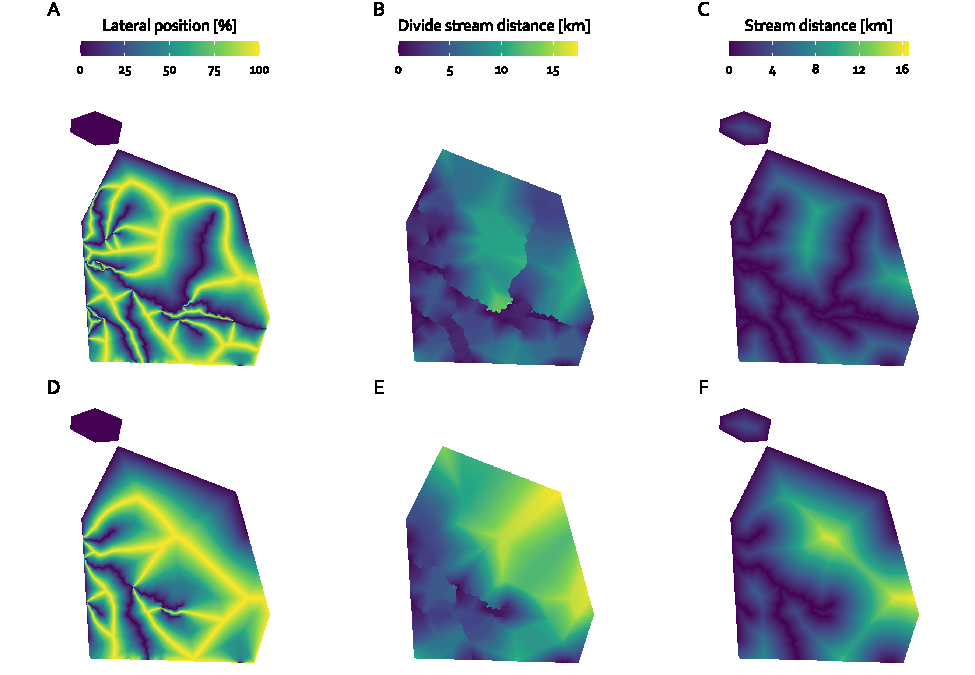
\includegraphics[width=1\linewidth]{data_descriptor/tex/figure-datasetmapoverviewplot-1} 

}

\caption{Resulting maps of the three EU-MOHP measures lateral position (A, D), divide stream distance (B, E) and stream distance (C, F) for the two hydrologic orders 3 (A, B, C) and 4 (D, E, F). The colour gradients in the legend represents the mapped values of all plots in its column.}\label{fig:datasetmapoverviewplot}
\end{figure}

\normalsize

\footnotesize

\begin{figure}[H]

{\centering 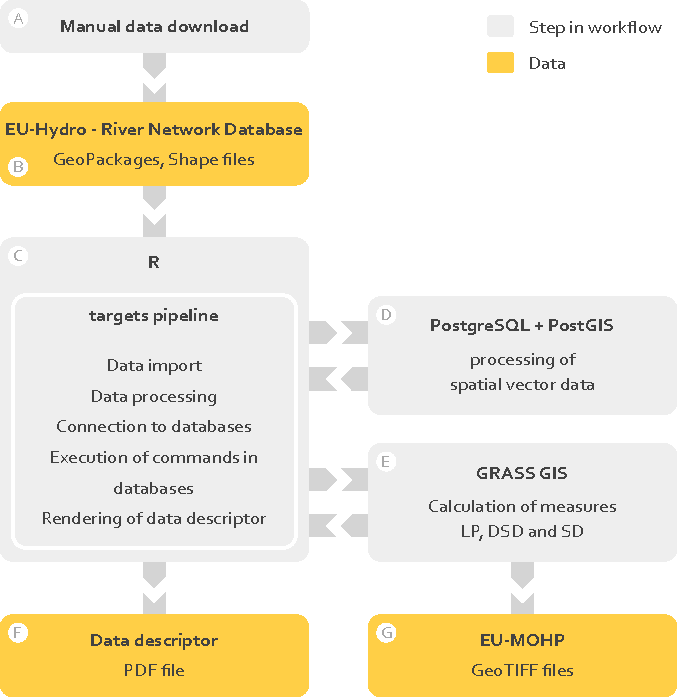
\includegraphics[width=0.7\linewidth]{data_descriptor/tex/workflow_figure} 

}

\caption{Workflow of the data processing in different software.}\label{fig:workflowfigure}
\end{figure}

\normalsize

\footnotesize

\begin{figure}[H]

{\centering 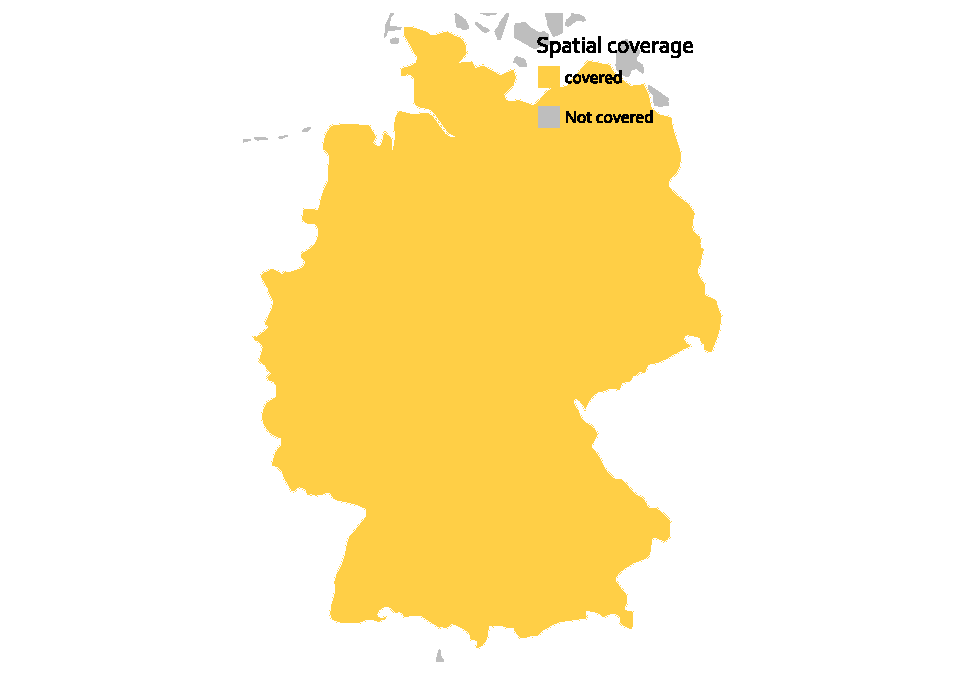
\includegraphics[width=1\linewidth]{data_descriptor/tex/figure-studyareafigure-1} 

}

\caption{Spatial coverage of this dataset. The legend labels show the names according to the outpu file name. If you want to check more precisely whether your study area or area of interest is covered by this dataset, please visit !!link to github readme.}\label{fig:studyareafigure}
\end{figure}

\normalsize

\footnotesize

\begin{figure}[H]

{\centering 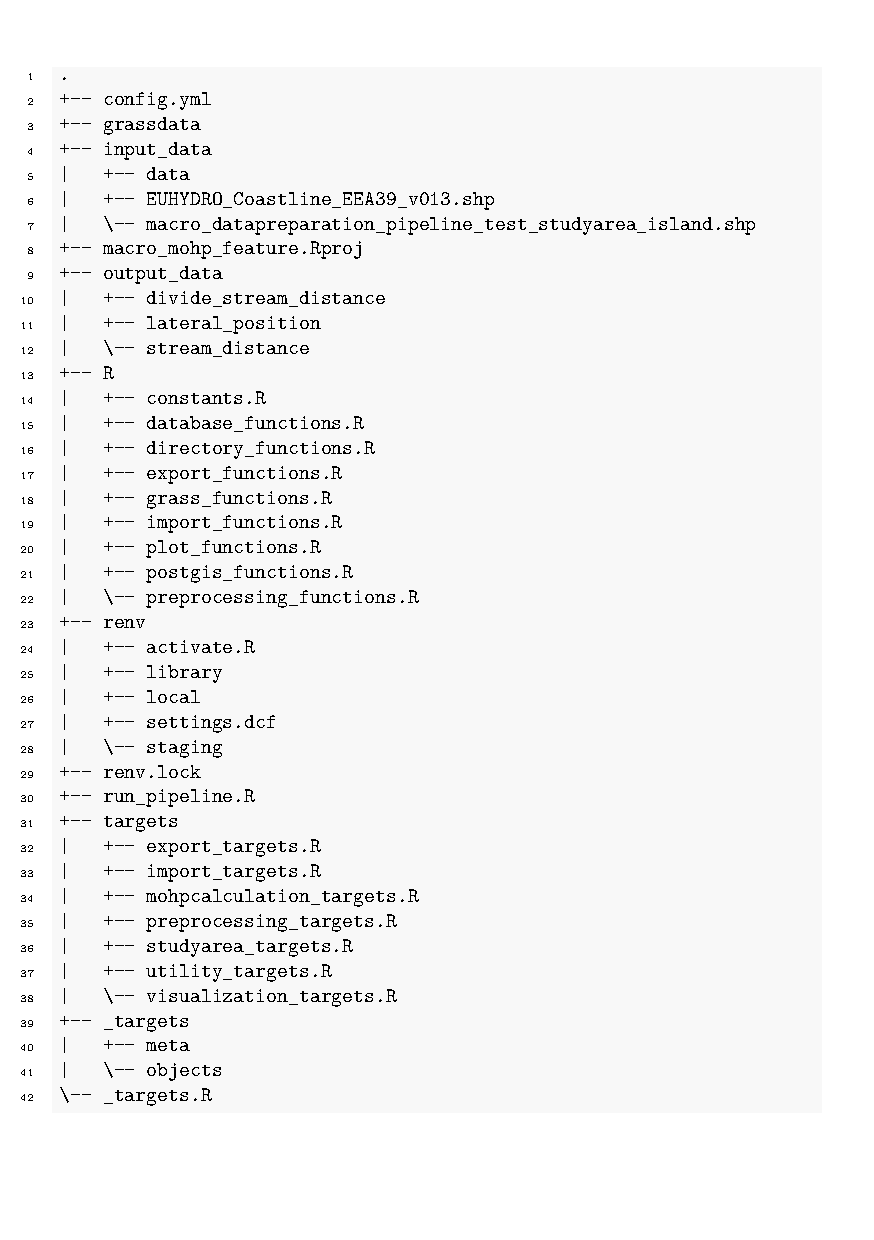
\includegraphics[width=0.7\linewidth]{data_descriptor/tex/directory_tree} 

}

\caption{Directory tree of the project directory; only relevant subdirectories and files are listed here.}\label{fig:projectdirtree}
\end{figure}

\normalsize

\footnotesize

\begin{figure}[H]

{\centering 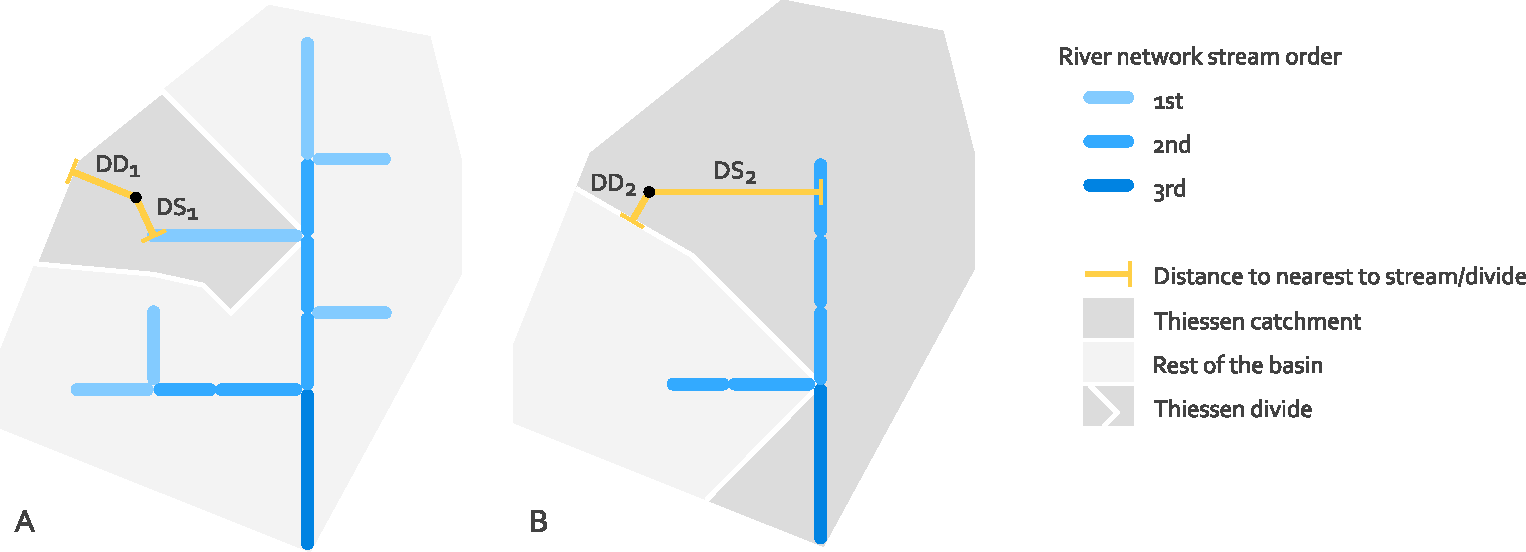
\includegraphics[width=1\linewidth]{data_descriptor/tex/mohp_scheme} 

}

\caption{Schematic representation of MOHP measures using two examples for the hydrologic orders 1 (A) and 2 (B).}\label{fig:schematicmohp}
\end{figure}

\normalsize

\footnotesize

\begin{figure}[H]

{\centering 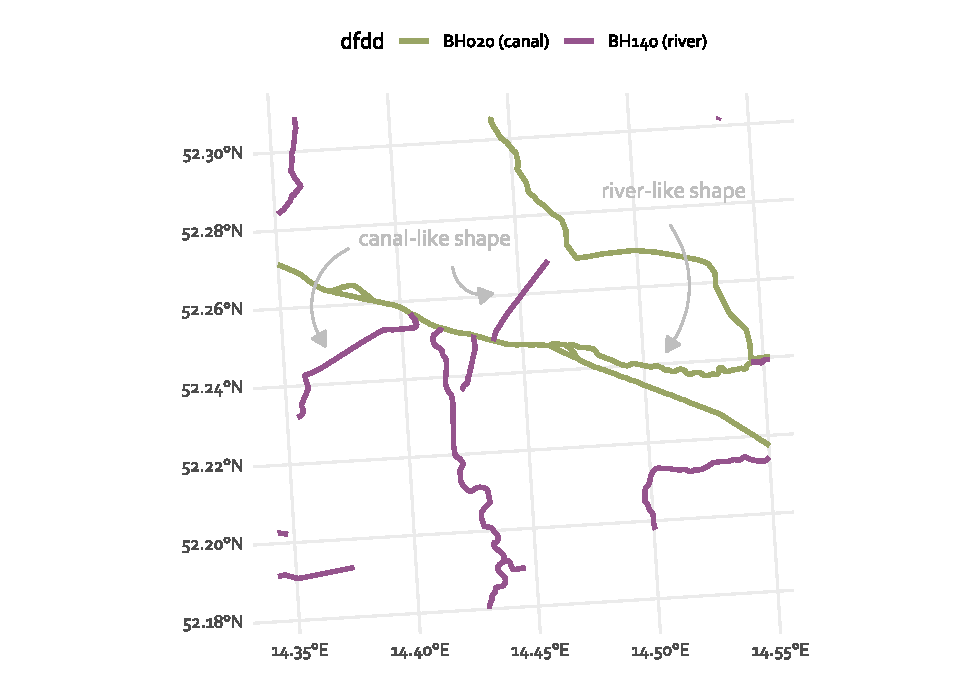
\includegraphics[width=0.8\linewidth]{data_descriptor/tex/figure-rivercanalconfusionplot-1} 

}

\caption{Example of the river network data showing the confusion between the classes BH140 (river), BH020 (canal) and BH030 (ditch).}\label{fig:rivercanalconfusionplot}
\end{figure}

\normalsize

\footnotesize

\begin{figure}[H]

{\centering 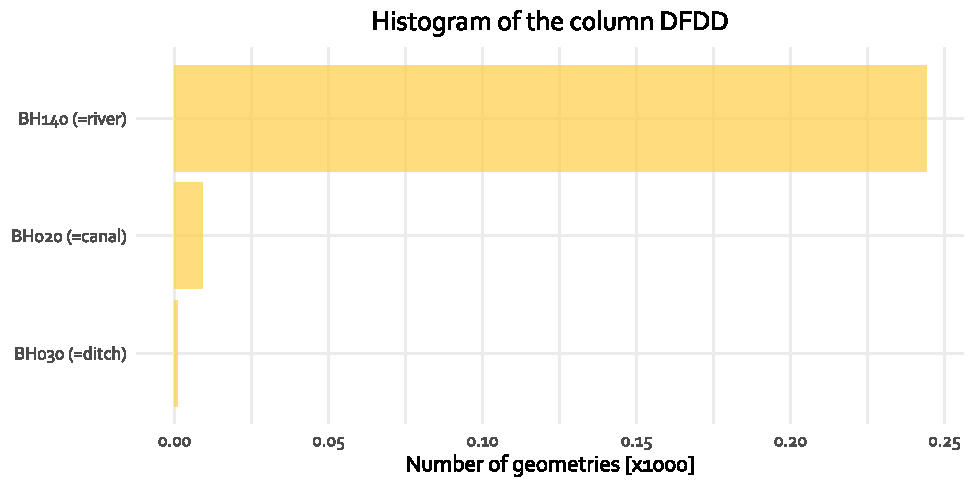
\includegraphics[width=0.8\linewidth]{data_descriptor/tex/figure-dfddstatsbarplot-1} 

}

\caption{Distribution of classes BH140 (river), BH020 (canal) and BH030 (ditch) of the attribute column "DFDD".}\label{fig:dfddstatsbarplot}
\end{figure}

\normalsize

\footnotesize

\begin{figure}[H]

{\centering 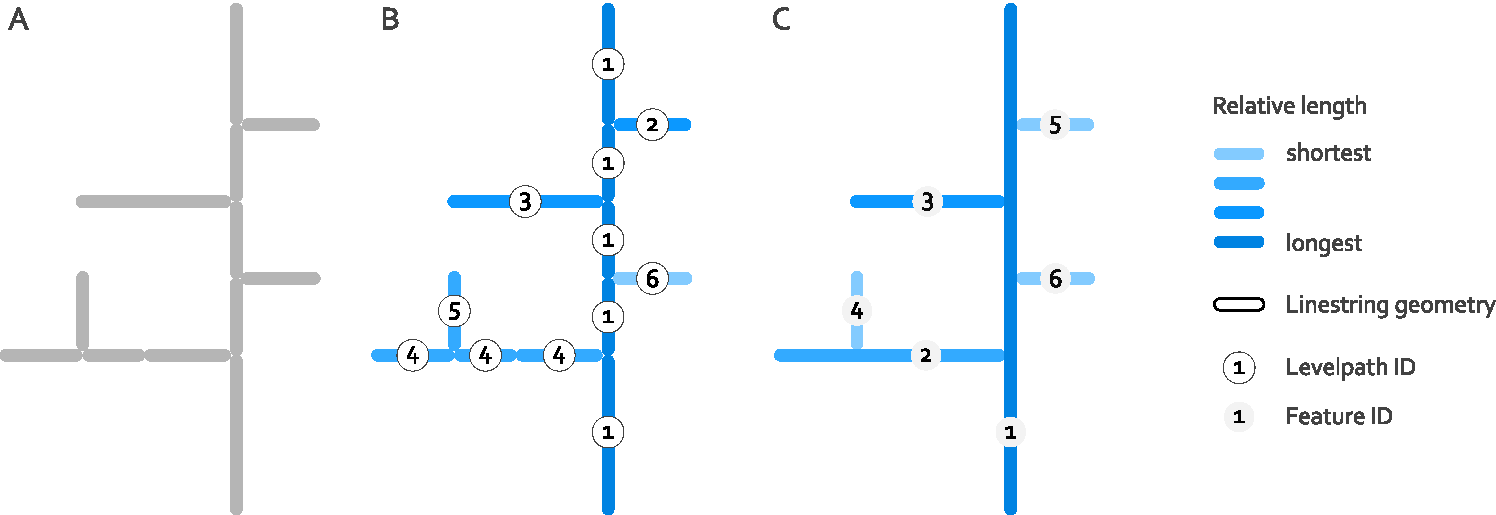
\includegraphics[width=1\linewidth]{data_descriptor/tex/mainstem_scheme} 

}

\caption{Schematic representation of the river network and its linestring geometries after import (A), after the identification of mainstems including the column `Levelpath ID` (B) and after merging the linestring geometries by this column and adding a `Feature ID` column (C).}\label{fig:mainstemscheme}
\end{figure}

\normalsize

\footnotesize

\begin{figure}[H]

{\centering 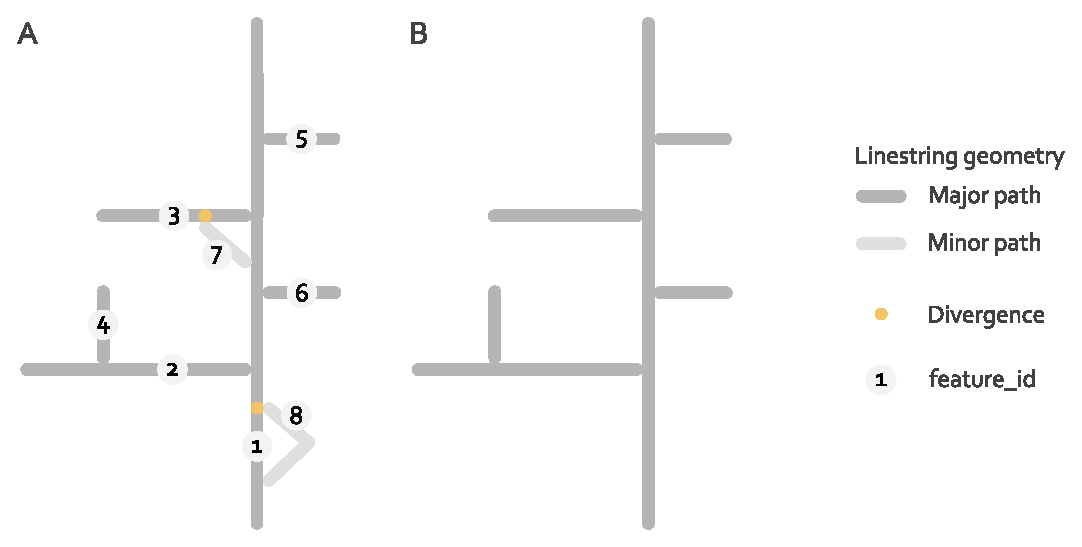
\includegraphics[width=1\linewidth]{data_descriptor/tex/divergences_scheme} 

}

\caption{Schematic representation of the river network and its linestring geometries inlcuding divergences before (A) and after (B) the removal of minor paths under the condition that they intersect with the same linestring geometry at the start and end node. The linestring geometry with the "Feature ID" 8 is being removed from the river network in B, because it intersects the linestring geometry with the ID 1 the start and end node. Whereas linestring geometry with the ID 7 remains in the river network, because it intersects with two different linestring geometries at start and end node (ID 3 and ID 1).}\label{fig:divergencescheme}
\end{figure}

\normalsize

\footnotesize

\begin{figure}[H]

{\centering 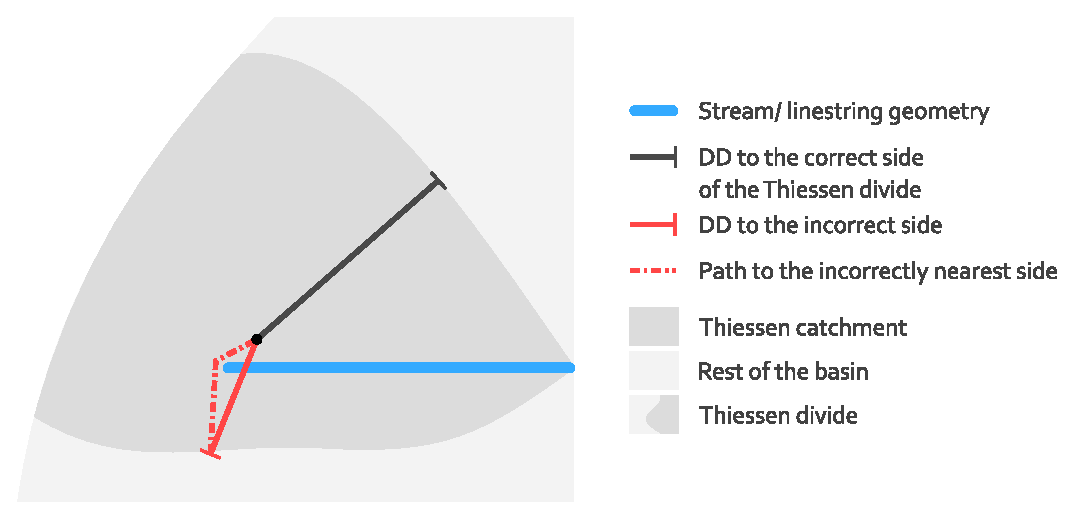
\includegraphics[width=0.7\linewidth]{data_descriptor/tex/dd_inaccuracies} 

}

\caption{Schematic example showing the source of inaccurate of DD in areas near headwaters caused by the applied method to calculate DD. The red distance as DD is incorrect, because it crosses the stream and therefore does not fulfill the defined condition  The correct DD would be the green distance.}\label{fig:ddinaccuracies}
\end{figure}

\normalsize

\footnotesize

\begin{table}

\caption{\label{tab:runtime}Overview of the run-time and data size of all targets or processing steps in descending order.}
\centering
\begin{tabu} to \linewidth {>{\raggedright\arraybackslash}p{20em}>{\raggedleft}X>{\raggedleft}X>{\raggedleft}X>{\raggedleft}X>{\raggedleft}X}
\toprule
\multicolumn{1}{c}{ } & \multicolumn{4}{c}{Run-time} & \multicolumn{1}{c}{Data size} \\
\cmidrule(l{3pt}r{3pt}){2-5} \cmidrule(l{3pt}r{3pt}){6-6}
Target name & Seconds & Minutes & Hours & Days & Mb\\
\midrule
river\_networks & 965.3 & 16.1 & 0.3 & 0 & 1112.0\\
inland\_waters & 181.5 & 3.0 & 0.1 & 0 & 183.0\\
db\_objects\_to\_grass & 167.5 & 2.8 & 0.0 & 0 & 0.0\\
data\_descriptor & 46.4 & 0.8 & 0.0 & 0 & 1.9\\
river\_canal\_confusion\_plot & 40.0 & 0.7 & 0.0 & 0 & 1112.2\\
\addlinespace
river\_networks\_clip & 39.9 & 0.7 & 0.0 & 0 & 0.3\\
db\_inland\_waters & 23.1 & 0.4 & 0.0 & 0 & 0.0\\
rivernetworks\_merged\_per\_streamorder & 7.3 & 0.1 & 0.0 & 0 & 0.7\\
dataset\_map\_overview\_plot & 8.4 & 0.1 & 0.0 & 0 & 71.4\\
directory\_tree & 7.8 & 0.1 & 0.0 & 0 & 0.0\\
\addlinespace
workflow\_figure & 7.7 & 0.1 & 0.0 & 0 & 0.0\\
input\_data\_table & 7.3 & 0.1 & 0.0 & 0 & 0.0\\
selected\_hydrologic\_orders & 7.2 & 0.1 & 0.0 & 0 & 0.0\\
river\_networks\_streamorderone & 7.1 & 0.1 & 0.0 & 0 & 0.3\\
distinct\_streamorders\_in\_riverbasins & 5.6 & 0.1 & 0.0 & 0 & 0.0\\
\addlinespace
filepath\_studyarea\_pipelinetest & 5.4 & 0.1 & 0.0 & 0 & 0.0\\
config & 5.2 & 0.1 & 0.0 & 0 & 0.0\\
directory\_river\_networks & 4.5 & 0.1 & 0.0 & 0 & 0.0\\
river\_basin\_names & 4.4 & 0.1 & 0.0 & 0 & 0.0\\
db\_river\_networks\_merged\_per\_streamorder & 5.8 & 0.1 & 0.0 & 0 & 0.0\\
\addlinespace
db\_inland\_waters\_strahler & 1.8 & 0.0 & 0.0 & 0 & 0.0\\
studyarea\_figure & 1.0 & 0.0 & 0.0 & 0 & 0.2\\
db\_selected\_studyarea & 0.7 & 0.0 & 0.0 & 0 & 0.0\\
rivernetworks\_feature\_id & 1.4 & 0.0 & 0.0 & 0 & 0.7\\
selected\_studyarea & 0.6 & 0.0 & 0.0 & 0 & 0.0\\
\addlinespace
db\_river\_networks\_strahler\_studyarea & 0.4 & 0.0 & 0.0 & 0 & 0.0\\
db\_river\_networks\_clean & 0.4 & 0.0 & 0.0 & 0 & 0.0\\
coastline\_watershed & 0.4 & 0.0 & 0.0 & 0 & 0.0\\
output\_data\_table & 0.1 & 0.0 & 0.0 & 0 & 0.0\\
dfdd\_stats\_bar\_plot & 0.0 & 0.0 & 0.0 & 0 & 0.4\\
\addlinespace
river\_networks\_files & 0.0 & 0.0 & 0.0 & 0 & 0.0\\
river\_networks\_greater\_one\_grouped & 0.0 & 0.0 & 0.0 & 0 & 0.4\\
streamorders & 0.0 & 0.0 & 0.0 & 0 & 0.0\\
river\_networks\_grouped & 0.0 & 0.0 & 0.0 & 0 & 0.7\\
river\_networks\_non\_dry\_selected\_streamtypes & 0.0 & 0.0 & 0.0 & 0 & 0.3\\
\addlinespace
river\_networks\_clean & 0.0 & 0.0 & 0.0 & 0 & 0.3\\
river\_networks\_treated\_brackets & 6.0 & 0.1 & 0.0 & 0 & 0.0\\
river\_networks\_imputed\_streamorder\_canals\_as\_1 & 0.0 & 0.0 & 0.0 & 0 & 0.3\\
\midrule
\textbf{Total} & \textbf{1560.2} & \textbf{25.9} & \textbf{0.4} & \textbf{0} & \textbf{2485.1}\\
\bottomrule
\end{tabu}
\end{table}

\normalsize

\footnotesize

\begin{table}

\caption{\label{tab:outputdata}Overview of the output file naming scheme and its placeholder values. Files for any combinations of the placeholder values exists. The values are inserted for the respective placeholder in "mohp\_europe\_<region name for spatial coverage>\_<abbreviation of the EU-MOHP measure>\_<hydrologic order>\_<spatial resolution>.tif". For example, selecting the first value of each placeholder results in the file name "mohp\_europe\_europemainland\_dsd\_streamorder1\_30m.tif". The spatial coverage of the values for "<region name for spatial coverage>" is shown in Fig. 1.}
\centering
\begin{tabu} to \linewidth {>{\raggedright}X>{\raggedright\arraybackslash}p{12em}>{\raggedright}X}
\toprule
Placeholder in output file name & Value & Description\\
\midrule
 & europemainland & Raster data covers the contiguous land area of continental Europe, ...\\
\cmidrule{2-3}
 & finland-norway-sweden & ...the Scandinavian countries Finland, Norway and Sweden\\
\cmidrule{2-3}
 & france & ...Corsica\\
\cmidrule{2-3}
 & greece & ...Creta\\
\cmidrule{2-3}
 & iceland & ...Iceland\\
\cmidrule{2-3}
 & italy1 & ...Sicily\\
\cmidrule{2-3}
 & italy2 & ...Sardinia\\
\cmidrule{2-3}
 & turkey & ...Turkey\\
\cmidrule{2-3}
 & unitedkingdom & ...United Kingdom\\
\cmidrule{2-3}
\multirow{-10}{*}{\raggedright\arraybackslash <region name for spatial coverage>} & unitedkingdom-ireland & Ireland and North Ireland\\
\cmidrule{1-3}
 & dsd & Divide stream distance\\
\cmidrule{2-3}
 & lp & Lateral Position\\
\cmidrule{2-3}
\multirow{-3}{*}{\raggedright\arraybackslash <abbreviation of the EU-MOHP measure>} & sd & Stream distance\\
\cmidrule{1-3}
 & streamorder1 & \\
\cmidrule{2-2}
 & streamorder2 & \\
\cmidrule{2-2}
 & streamorder3 & \\
\cmidrule{2-2}
 & streamorder4 & \\
\cmidrule{2-2}
 & streamorder5 & \\
\cmidrule{2-2}
\multirow{-6}{*}{\raggedright\arraybackslash <hydrologic order>} & streamorder6 & \multirow{-6}{*}{\raggedright\arraybackslash Hydrologic order}\\
\cmidrule{1-3}
<spatial resolution> & 30m & Spatial resolution\\
\bottomrule
\end{tabu}
\end{table}

\normalsize

\FloatBarrier

\nocite{*}
\bibliography{eu-mohp.bib}

\end{document}
